%!TEX encoding = UTF-8 Unicode

\section{Experimental Results}

In this section, we report the experimental findings obtained with our proposed model.
%when using information originating from the observation of an external agent~(human).
We present the following types of results:
\begin{itemize}
  \item inferences over affordance variables~(i.e., the entries of Table~\ref{tab:bnsymb} except the last row therein);

  \item predictions of word probabilities~(i.e., the last row of Table~\ref{tab:bnsymb});

  \item generated verbal descriptions from the word probabilities of the previous point, according to a formal grammar. The descriptions, in turn, can be interpreted to observe the emergence of certain language phenomena~(e.g., choice of most appropriate conjunction word, choice of synonym words between two consecutive sentences when they refer to the same object).
\end{itemize}

% Giampiero: I would remove this because it not surprising and a bit confusing. We would need to explain for example why touch has so low probability in the absence of any evidence (this is actually surpising to me). It might make more sense if we gave evidence to the BN that is contrary to the HMM evidence.
\subsection{Inference over Affordance Variables (Including Action, Synthetic Values)}

\begin{figure}
\centering
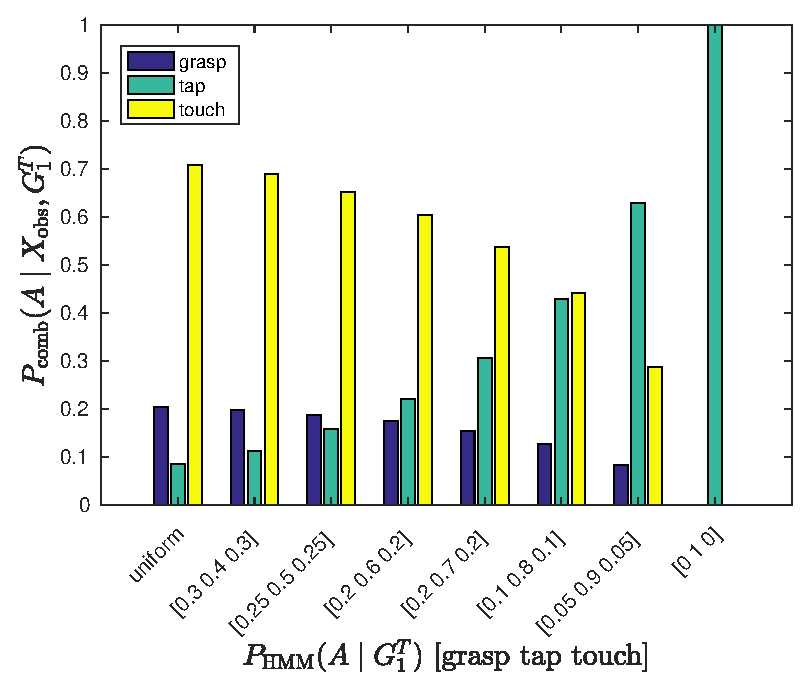
\includegraphics[width=0.9\columnwidth]{impact_of_evidence_on_Action.eps}
\caption{Predictions about the action over a big sphere, when given different probabilistic soft evidence about the action.}
\label{fig:impact_of_evidence_on_Action}
\end{figure}

%We now report a result that uses the \emph{soft decision} from the Gesture \acp{HMM}, i.e., the probability distribution over the possible actions.
In Fig.~\ref{fig:impact_of_evidence_on_Action} we show compactly the result of eight different queries~(each group of bars), corresponding to the same number of eight different soft evidences over the action, ranging from a non-informative, uniform distribution~(i.e.,~[1/3~1/3~1/3]), up to the maximum score being attributed to the ``tap'' action~(i.e.,~[0~1~0]), with intermediate distributions in between.
The resulting posterior probability over the Action node is initially ambiguous between ``grasp'' and ``tap'', but then it becomes more and more polarized towards the ``tap'' action as our prior becomes more informative.
This result is not surprising, because the Action node is used both as a prior and as a posterior.
Nonetheless, it serves to validade our formulation for combining different sources of information~(see Sec.~\ref{sec:combination}).

\subsection{Inference over Affordance Variables (Excluding Action, Synthetic Values)}

\begin{figure*}
\centering
\subfloat[][Predictions about the object velocity of a sphere, when given different probabilistic soft evidence about the action.]
{ 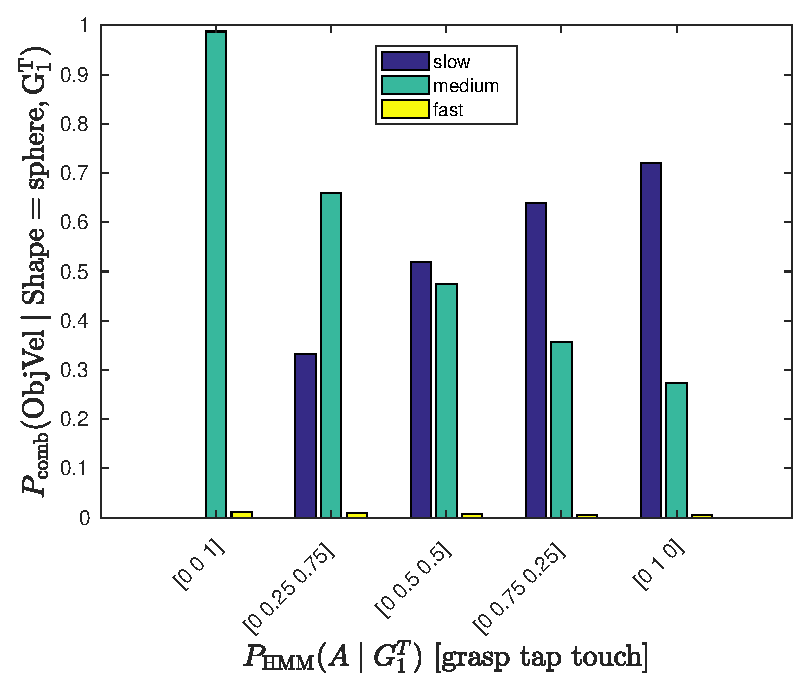
\includegraphics[width=0.45\linewidth]{impact_of_evidence_on_ObjVel_sphere.eps} \label{fig:impact_of_evidence_on_ObjVel_sphere} } \quad
%
\subfloat[][Predictions about the object velocity of a box, when given different probabilistic soft evidence about the action.]
{ 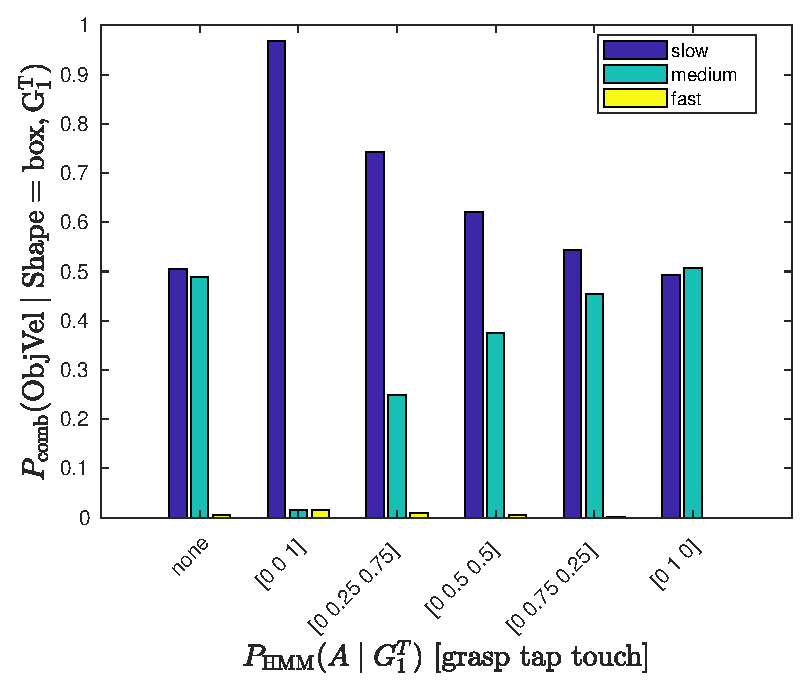
\includegraphics[width=0.45\linewidth]{impact_of_evidence_on_ObjVel_box.eps} \label{fig:impact_of_evidence_on_ObjVel_box} }
\caption{Predictions about the object velocity of different objects, when given probabilistic soft evidence about the action.}
\label{fig:impact_of_evidence_on_ObjVel}
\end{figure*}

Next, we report a result that also uses the \emph{soft decision} over the Action node from the Gesture \acp{HMM}, but this time makes a prediction over a different node: object velocity~(which expresses an effect information).
Fig.~\ref{fig:impact_of_evidence_on_ObjVel} shows the inference in two cases: when the prior information says that the shape is spherical~(see Fig.~\ref{fig:impact_of_evidence_on_ObjVel_sphere}), and when it is cubic~(see Fig.~\ref{fig:impact_of_evidence_on_ObjVel_box}).
TODO complete

\subsection{Inference over Affordance Variables (Excluding Action, Real Values)}

% RESULT FROM GLU WITH HARD EVIDENCE
%
% {\color{red}
% Giampiero: in this example we should: 1) not use hard evidence, but soft 2) base the evidence on some of the recorded examples of tap. I believe the same results would be obtained given that the ti evidence from the HMM is not completely random.
% }

Because it is based on \ac{BN}, our model can make predictions over any set of its variables, given any other set of observed variables.
In particular, the model can do reasoning on the elements that constitute our computational concept of affordances, i.e., Action, Object Features, Effects in Fig.~\ref{fig:model}.
For example, we can reason about the expected object velocity effects that an action will cause onto environment objects, in an anticipatory fashion, thus computing~\eqref{eq:fusion_excluding_action}.
Note that the estimation of the human action,~$\phmm(A \given G_1^N)$, is a \emph{soft decision}, meaning that it represents the~(time-evolving) probability distribution over the possible actions.
Fig.~\ref{fig:effect_pred_sphere} shows the experiment when the human performs an action onto a small spherical object, whereas Fig.~\ref{fig:effect_pred_box} displays it when the object is a big box.

%\begin{figure*}
%    \centering
%    \subfloat[][Evolution of the action posterior in time, using~\eqref{eq:phmm_action}.]{
%      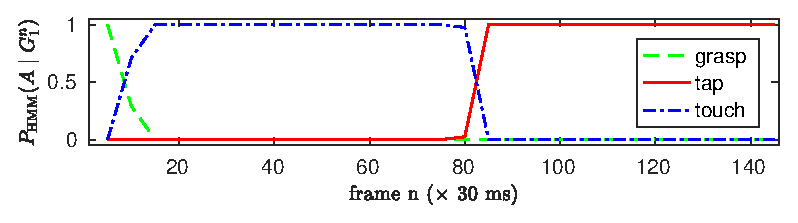
\includegraphics[width=0.7\linewidth]{evolution_of_action_posterior_on_sphere.eps}
%      \label{fig:effect_pred_sphere:action_posterior_evolution}
%    }
%
%    \subfloat[][First three photos: observation of human agent performing the action. Right: prediction of the movement effect.]{
%      % TODO purge old pics from repo if not used
%      %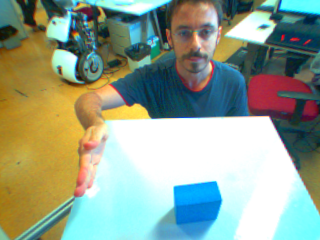
\includegraphics[width=\myWidth\linewidth]{tap-00000109}
%      %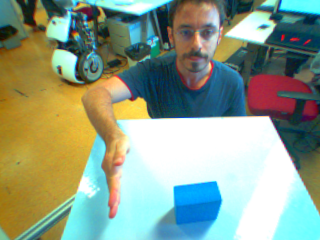
\includegraphics[width=\myWidth\linewidth]{tap-00000110}
%      %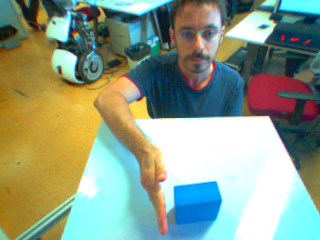
\includegraphics[width=\myWidth\linewidth]{tap-00000112}
%      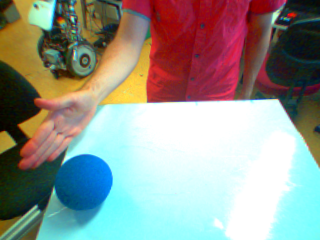
\includegraphics[width=\myWidth\linewidth]{tap-sphere-00000179}
%      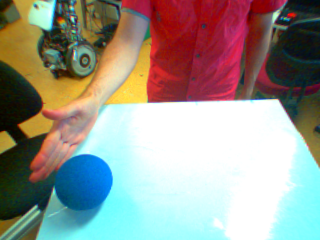
\includegraphics[width=\myWidth\linewidth]{tap-sphere-00000183}
%      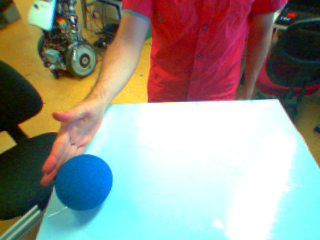
\includegraphics[width=\myWidth\linewidth]{tap-sphere-00000187}
%      \quad
%      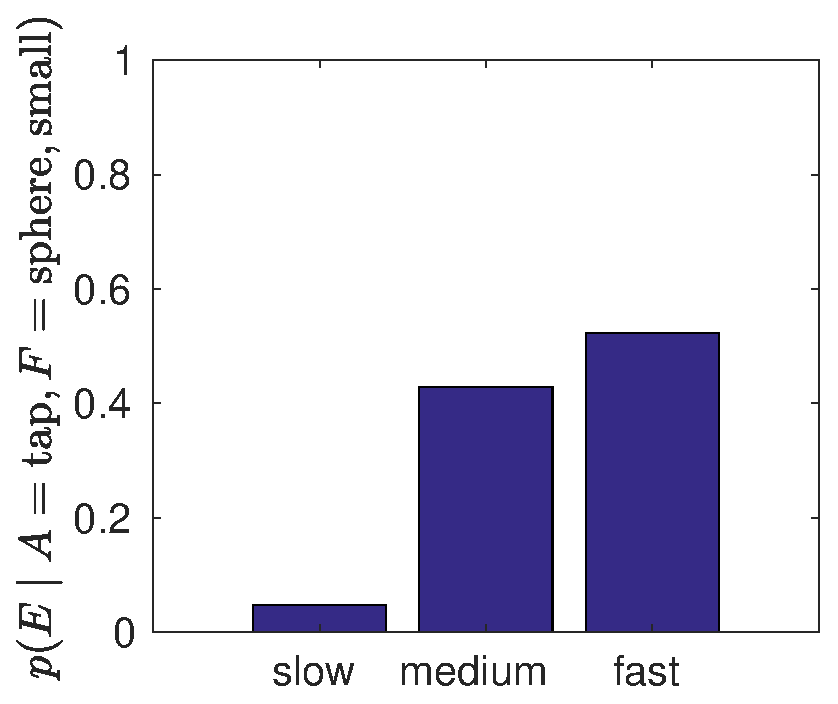
\includegraphics[width=0.20\linewidth]{effectpred_sphere.eps}
%      \label{fig:effect_pred_sphere:observation_and_prediction}
%    }
%
%    \caption{Object velocity predictions on a small sphere, given probabilistic human action information from Gesture \acp{HMM}.}
%    \label{fig:effect_pred_sphere}
%\end{figure*}

In~\ref{fig:effect_pred_sphere:action_posterior_evolution}, we visualize the temporal evolution of the human action posterior probability distribution, as computed by the Gesture/Action Recognition algorithm when the human is moving the hand, before the contact to the object is made~(see Fig.~\ref{fig:effect_pred_sphere:observation_and_prediction}, first three photos).
After about two thirds of the human movement have been completed, the model guesses correctly that it is a tap movement.
(Before that instant, the model guesses the wrong action, in addition doing it with certainty, due to the way that the individual gestures have been modeled by continuous mixtures of Gaussian values GIAMPIERO PLEASE CHECK THIS.)
In Fig.~\ref{fig:effect_pred_sphere:observation_and_prediction}~(rightmost plot), we show the final prediction of the moment effect on the small sphere.
In essence, the combined model has predicted that this target object will exhibit a medium or fast velocity after the human will touch it.

\begin{figure*}
  \begin{tikzpicture}
    \node (lik) {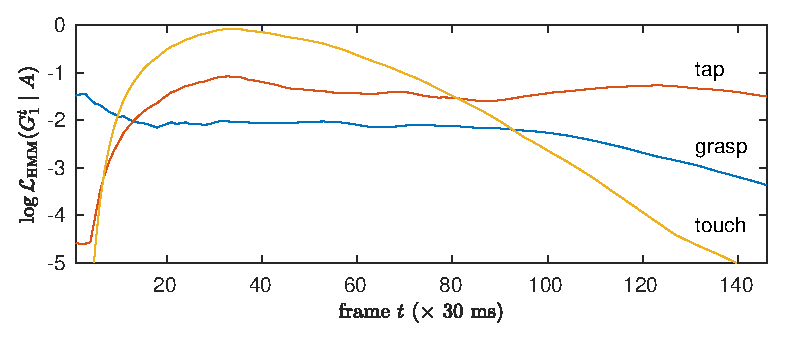
\includegraphics[width=0.6\linewidth]{evolution_of_action_posterior_box_log.eps}};
    \node at ([xshift=-90pt,yshift=30pt]lik.north) {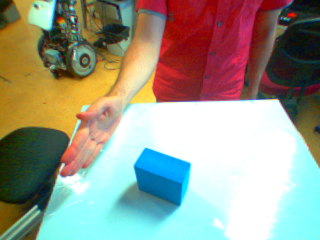
\includegraphics[width=\myWidth\linewidth]{tap-box-00000230}};
    \node at ([xshift=+10pt,yshift=30pt]lik.north) {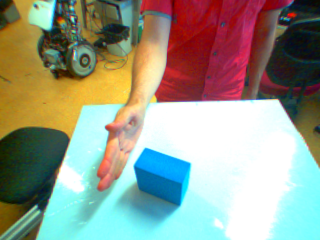
\includegraphics[width=\myWidth\linewidth]{tap-box-00000250}};
    \node at ([xshift=+110pt,yshift=30pt]lik.north) {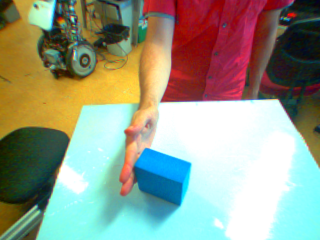
\includegraphics[width=\myWidth\linewidth]{tap-box-00000270}};
  \end{tikzpicture}
  \quad
  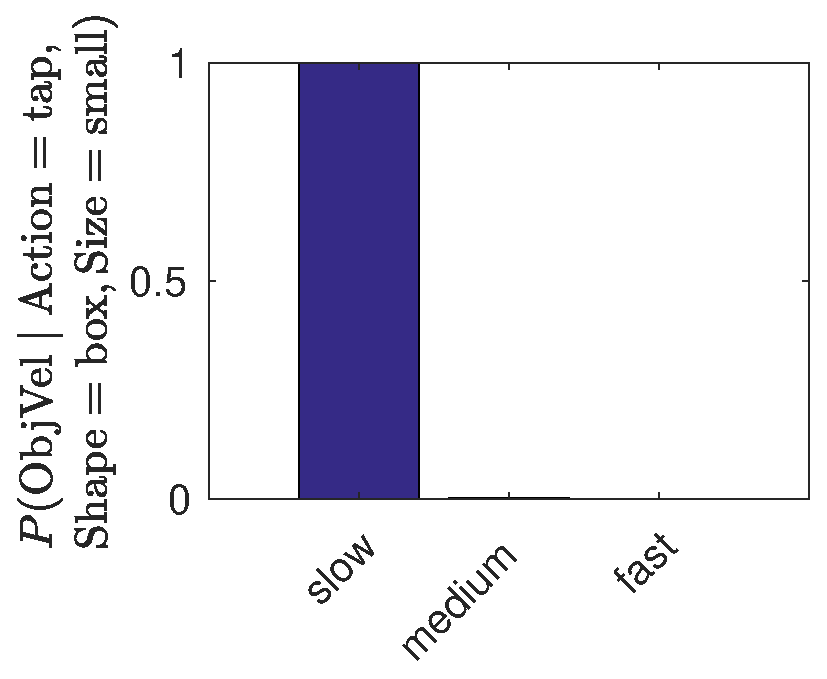
\includegraphics[width=0.35\linewidth]{effectpred_box.eps}
  \caption{Object velocity predictions on a big box, given probabilistic human action information from Gesture \acp{HMM}.}
  \label{fig:effect_pred_box}
\end{figure*}

\begin{figure*}
  \begin{tikzpicture}
    \node (lik) {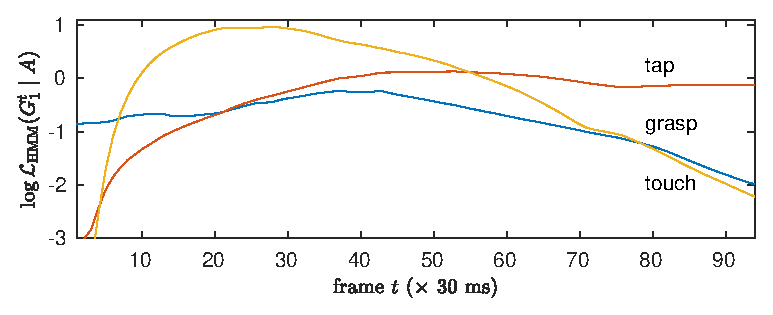
\includegraphics[width=0.6\linewidth]{evolution_of_action_posterior_sphere_log.eps}};
    \node at ([xshift=-90pt,yshift=30pt]lik.north) {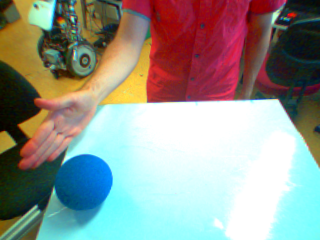
\includegraphics[width=\myWidth\linewidth]{tap-sphere-00000179}};
    \node at ([xshift=+10pt,yshift=30pt]lik.north) {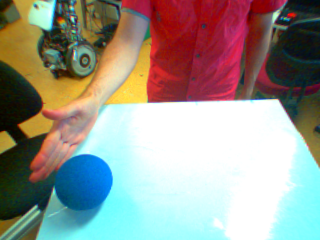
\includegraphics[width=\myWidth\linewidth]{tap-sphere-00000183}};
    \node at ([xshift=+110pt,yshift=30pt]lik.north) {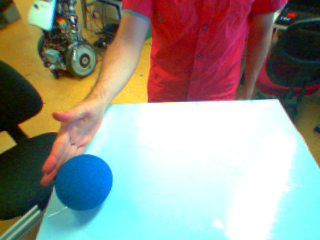
\includegraphics[width=\myWidth\linewidth]{tap-sphere-00000187}};
  \end{tikzpicture}
  \quad
  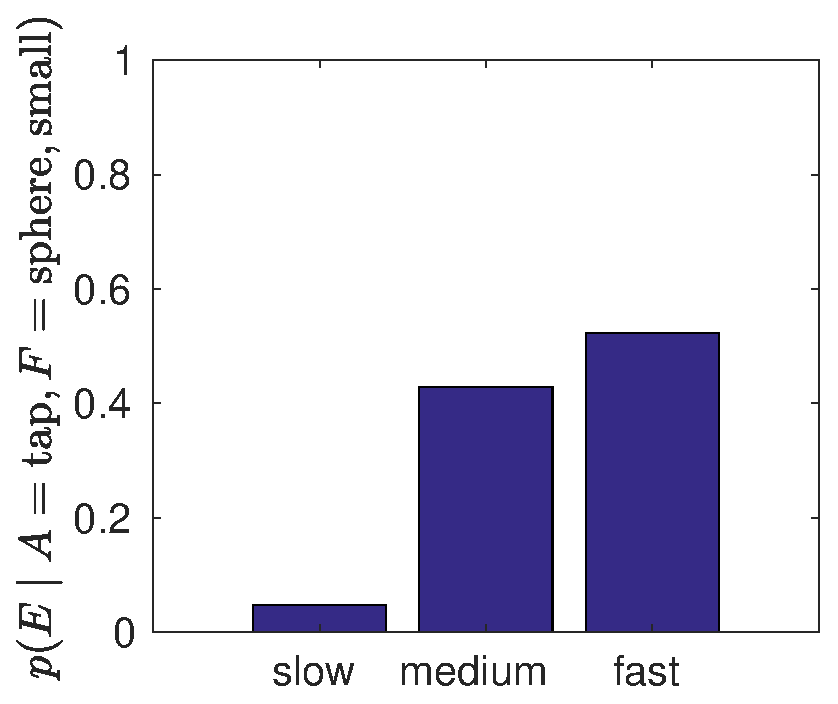
\includegraphics[width=0.35\linewidth]{effectpred_sphere.eps}
  \caption{Object velocity predictions on a small sphere, given probabilistic human action information from Gesture \acp{HMM}.}
  \label{fig:effect_pred_sphere}
\end{figure*}

%\begin{figure*}
%    \centering
%    \subfloat[][Evolution of the action posterior in time, using~\eqref{eq:phmm_action}.]{
%      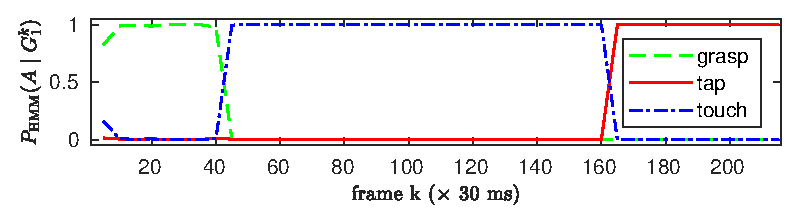
\includegraphics[width=0.7\linewidth]{evolution_of_action_posterior_on_box.eps}
%      \label{fig:effect_pred_box:action_posterior_evolution}
%    }
%
%    \subfloat[][First three photos: observation of human agent performing the action. Right: prediction of the movement effect.]{
%      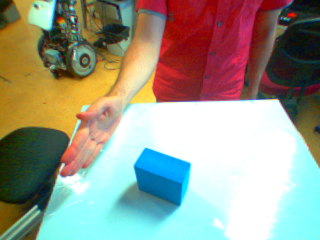
\includegraphics[width=\myWidth\linewidth]{tap-box-00000230}
%      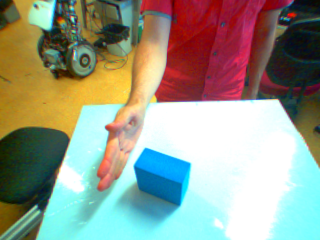
\includegraphics[width=\myWidth\linewidth]{tap-box-00000250}
%      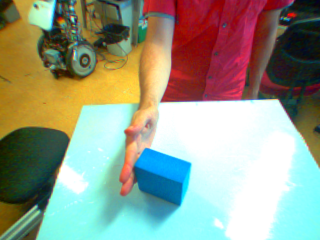
\includegraphics[width=\myWidth\linewidth]{tap-box-00000270}
%      \quad
%      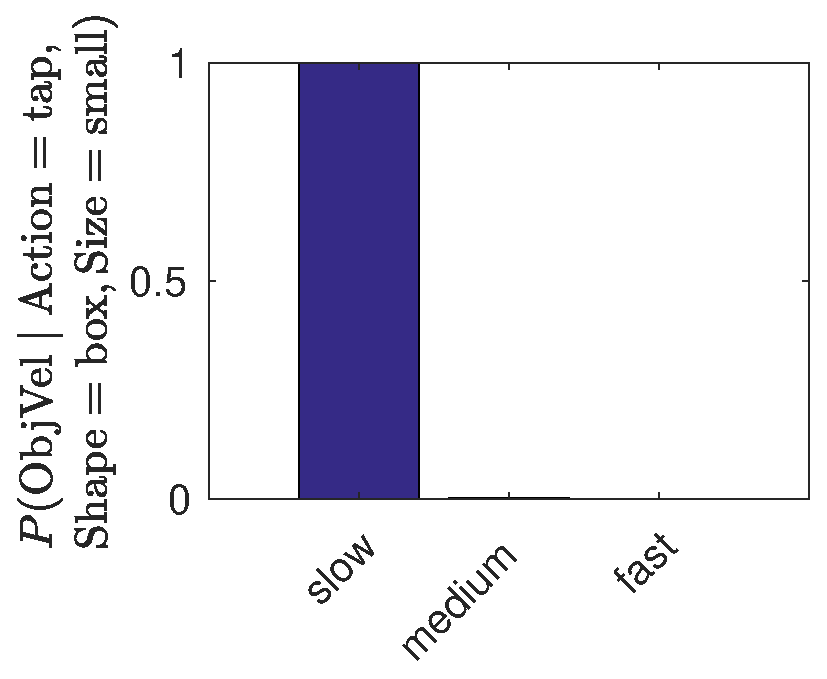
\includegraphics[width=0.20\linewidth]{effectpred_box.eps}
%      \label{fig:effect_pred_box:observation_and_prediction}
%    }
%
%    \caption{Object velocity predictions on a big box, given probabilistic human action information from Gesture \acp{HMM}.}
%    \label{fig:effect_pred_box}
%\end{figure*}

As for the experiment with the big box, Fig.~\ref{fig:effect_pred_sphere:action_posterior_evolution} shows the temporal evolution of the human action posterior.
Similar considerations to the previous example apply: after about~$60$\% of the sequence has been observed, the Gesture/Action Recognition block estimates the tap correctly.
This time, when we fuse the human action estimation to the extracted Object Features, instants below the contact occurs~(Fig.~\ref{fig:effect_pred_box:observation_and_prediction}, first three photos), we get a different result than before, show in Fig.~\ref{fig:effect_pred_box:observation_and_prediction}~(rightmost plot): the combined model has predicted that the object will yield a movement of type ``slow'', meaning that it will not move at all, or move slowly.

These two cases have shown that, given similar human action priors~(i.e., lateral taps on a target object), the expected movement returned by the model is very different depending on the physical properties of the object.

\subsection{Prediction of Word Probabilities}

RESULT FROM GLU WITH HARD EVIDENCE

\begin{figure}
\centering
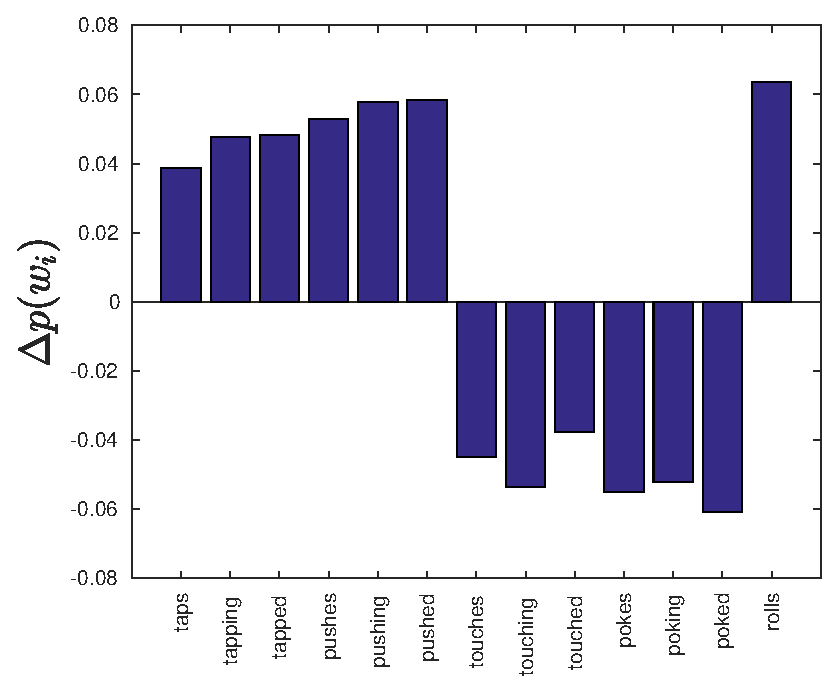
\includegraphics[width=0.9\columnwidth]{partialfig.eps}
\caption{Variation of word occurrence probabilities:
%$\Delta P(w_i) = P(w_i \mid \text{Size=big, Shape=sphere, ObjVel=fast, Action=tap}) - P(w_i \mid \text{Size=big, Shape=sphere,ObjVel=fast})$.
$\Delta P(w_i) = P(w_i \mid \text{InitialEvidence, Action=tap}) - P(w_i \mid \text{InitialEvidence})$, where $\text{InitialEvidence} = \{ \text{Size=big, Shape=sphere, ObjVel=fast} \}$.
This variation corresponds to the difference of word probability when we add the tap action evidence~(obtained from the Gesture \acp{HMM}) to the initial evidence about object features and effects. We have omitted words for which no significant variation was observed.}
\label{fig:probdiff}
\end{figure}

Our model permits to make predictions over the associated word descriptions in the presence or absence of an action prior.
%As in the previous experiment, we assume that the Gesture \acp{HMM} provide the discrete value of the recognized action performed by a human agent~(i.e., we enforce a hard decision over the observed action).
We compare the associated \emph{verbal description} obtained by the \acl{BN} in the absence of an action prior, with the ones obtained in the presence of one.
In particular, we compare the \emph{probability of word occurrence} resulting from the following two situations:
\begin{enumerate}
%\item when the robot prior knowledge~(evidence in the \ac{BN}) includes information about object features and effects only: \emph{Size=big, Shape=sphere, ObjVel=fast};
%\item when the robot prior knowledge includes, in addition to the above, evidence about the action as observed from the Gestures \acp{HMM}: \emph{Action=tap}.
\item robot prior knowledge evidence consisting of information about object features and effects only: %$\xobs^{\text{before}} = \{ \text{Size=big, Shape=sphere, ObjVel=fast} \}$;
\{Size=big, Shape=sphere, ObjVel=fast\};

\item prior evidence as in the previous situation, with the addition of the action observed from the Gestures \acp{HMM}: %$\xobs^{\text{after}} = \{ \text{Size=big, Shape=sphere, ObjVel=fast, Action=tap} \}$.
\{Size=big, Shape=sphere, ObjVel=fast, Action=tap\}.
\end{enumerate}

Fig.~\ref{fig:probdiff} shows the variation in word occurrence probabilities between the two cases, where we have omitted words for which no significant variation was observed.
We can interpret the difference in the predictions as follows: (i)~as expected, the probabilities of words related to tapping and pushing increase when a tapping action evidence from the Gestures \acp{HMM} is introduced; conversely, the probabilities of other action words~(touching and poking) decreases; (ii)~interestingly, the probability of the word \emph{rolling}~(which is an effect of an action onto an object) also increases when the tapping action evidence is entered. Even though the initial evidence of case~$1$ already included some effect information~(the velocity of the object), it is only now, when the robot perceives that the physical action was a tap, that the event rolling is associated.

\subsection{Verbal Descriptions}

In TODO ADD REF, we have seen how our model is able to generate word probabilities after having received probabilistic observed evidence.
In order to illustrate the capabilities of the model, we use the \ac{CFG} described in Appendix~\ref{appendix:grammar} to generate written descriptions of the robot observations on the basis of the probability distributions of the words inferred by the model.
Note that this grammar is defined here with the only purpose to interpret the probability distributions over the words.
The grammar was neither used in the speech recognition system, nor in learning the associations of the spoken utterances to the affordance variables.
In the model described in~\cite{salvi:2012:smcb}, the speech recognizer used a free loop of words with uniform prior distribution over the words, and the Bayesian model used a bag-of-words assumption, thus disregarding any syntactic information about the spoken descriptions.

During the self-centered learning phase, the verbal descriptions described the agent of the observed actions as either ``the~robot'', ``he'', or ``Baltazar''.
Consequently, the \AffWords{} model learned by the robot includes those words.
In the current study, by merging the \AffWords{} model and the gesture/action recognition model, we allow the robot to reinterpret the concepts it has learned in the self-centered phase, but we do not add any new words to the model.
Consequently, the descriptions that the model generates when observing humans use the same words to describe the agent.

The textual descriptions are generated as follows: given some evidence~$\xobs$ that we provide to the model and some human observation features~$G_1^n$ extracted from frames~$1$ to~$n$, we extract the generated word probabilities
$P(w_i \given \xobs, G_1^n)$.
We generate~$N$ sentences randomly from the \ac{CFG} using the \texttt{HSGen} tool from HTK~\cite{young:htkbook}.
Then, the sentences are re-scored according to the log-likelihood of each word in the sentence, normalized by the length of the sentence:
\begin{equation} \label{eq:sentence_score}
  \text{score}(s_j \given \xobs, G_1^n) = \frac{1}{L_j} \sum_{k=1}^{L_j} \log P(w_{jk} \given \xobs, G_1^n),
\end{equation}
where~$s_j$ is the~$j$th sentence,~$L_j$ is the number of words in the sentence~$s_j$, and~$w_{jk}$ is the~$k$th word in the sentence~$s_j$.
Finally, an $N$-best list of possible descriptions is produced by sorting the scores.

For example, if we provide the following evidence to the model:
\begin{equation} \label{eq:evidence_example}
    \xobs = \{\text{Color=yellow, Size=big, Shape=sphere, ObjVel=fast}\},
\end{equation}
we obtain
%the word probabilities of Fig.~\ref{fig:example_pw} and
the sentences reported in Table~\ref{tab:example_generated_sentences}.
The higher the score, the better.
In many of these sentences, we note that (i)~the correct action-related verb ``taps'' is generated (in the initial evidence, no action information was present, only object features and effects information were), and (ii)~the object term ``ball'' or synonyms thereof~(e.g., ``sphere'') are used coherently, both in the first part of the sentence describing the action and in the second part describing the effect.

% \begin{figure}
% \centering
% 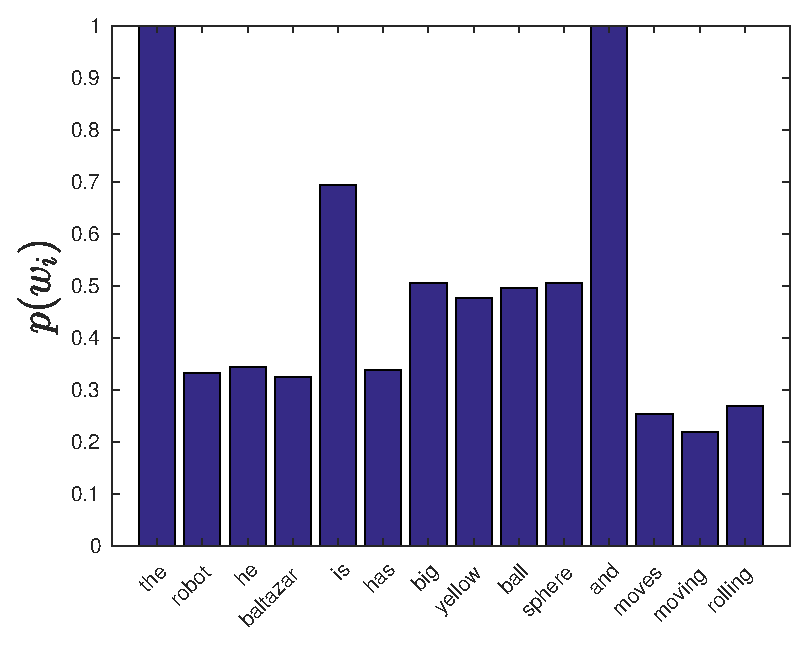
\includegraphics[width=0.9\columnwidth]{example_pw.eps}
% \caption{Word occurrence probabilities given the evidence \emph{\{Color=yellow, Size=big, Shape=sphere, ObjVel=fast\}}. We have omitted words for which no significant probability was observed.}
% \label{fig:example_pw}
% \end{figure}

\begin{table}
    \centering
    \caption{$10$-best list of sentences generated from the evidence~\eqref{eq:evidence_example}.}
    \label{tab:example_generated_sentences}
    \resizebox{\linewidth}{!}{% https://tex.stackexchange.com/a/27105/18819
    \begin{tabular}{ll}
    \toprule
    sentence & score \\
    \midrule
    the robot pushed the ball and the ball moves & $-0.54322$ \\ % not good to have push
    the robot tapped the sphere and the sphere moves & $-0.5605$ \\
    he is pushing the sphere and the sphere moves & $-0.57731$ \\
    the robot is tapping the yellow ball and the big yellow sphere is moving & $-0.57932$ \\
    he pushed the yellow ball and the sphere is rolling & $-0.58853$ \\
    the robot is poking the ball and the sphere is rolling & $-0.58998$ \\
    he is pushing the ball and the yellow ball moves & $-0.59728$ \\
    he pushes the sphere and the ball is moving & $-0.60528$ \\
    he is tapping the yellow ball and the ball is moving & $-0.60675$ \\
    the robot pokes the sphere and the ball is rolling & $-0.60694$ \\
    \bottomrule
    \end{tabular}%
    } % end resizebox
\end{table}

\subsection{Language Phenomenon: Choice of Correct Conjunction}

\newcommand{\evidenceProducingAnd}{Action=grasp, ObjVel=medium}
\newcommand{\evidenceProducingBut}{Action=grasp, ObjVel=slow}

The manipulation experiments that we consider have the following structure: an agent~(human or robot) performs a physical action onto an object with certain properties, and this object will produce a certain physical effect as a result.
For example, ``touch'' on an object yields no physical movement, but ``tap'' does~(especially if the object is spherical).
In the language description associated to an experiment, it makes sense to measure the conjunction chosen by the \acf{CFG} from the observed word probabilities.
In particular, it would be desirable to separate two kinds of behaviors: one in which the action and effect are coherent~(expected conjunction: ``and''), and the other one in which they are contradictory (``but'').

Fig.~\ref{tab:conjunction} shows an example of this behavior of the model.
We give the same action ``grasp'' to the model as evidence, but two values for the final object velocity.
When the object velocity is medium (Fig.~\ref{tab:conjunction:and}), the model interprets this as a successful grasp and uses the conjunction ``and'' to separate the description of the action from the description of the effect.
When the object velocity is slow (in the clustering procedure this was most often zero velocity), the model predicts this is an unsuccessful grasp and uses the conjunction ``but'', instead.

%Example in which the generated conjunction is ``and'' (because of consistency between nodes evidence):
%
%evidence:
%\begin{equation} \label{eq:evidence_producing_and}
%    \xobs^\prime = \{ \text{\evidenceProducingAnd} \}
%\end{equation}

%resulting word probabilities: Fig.~\ref{fig:conjunction_and:pw}

% \begin{figure}
% \centering
% 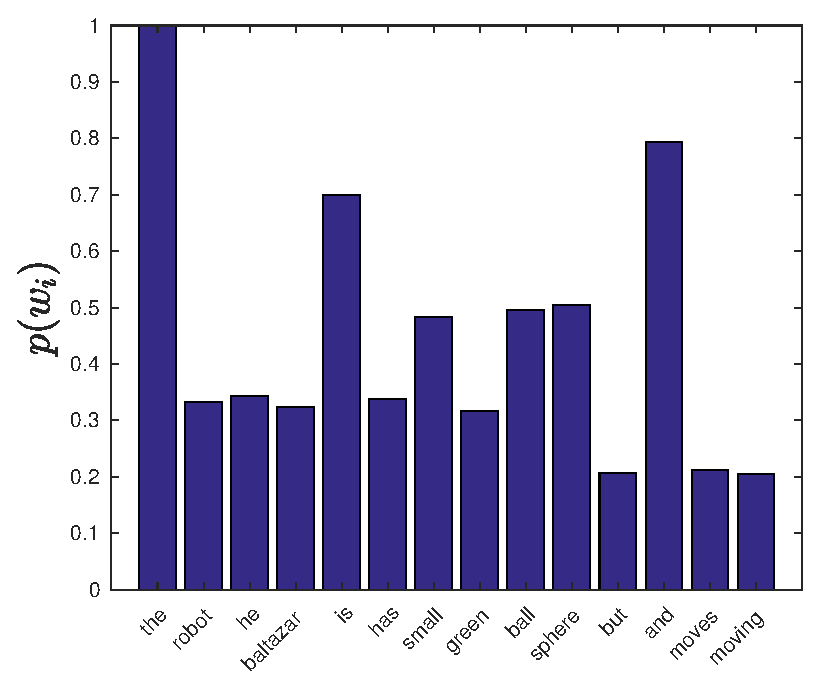
\includegraphics[width=0.9\columnwidth]{and_pw.eps}
% \caption{Word occurrence probabilities given the evidence \emph{\{\evidenceProducingAnd\}}. The ``and'' conjunction has a much higher probability than ``but''. See also Tab.~\ref{tab:conjunction:and}. We have omitted words for which no significant probability was observed.}
% \label{fig:conjunction_and:pw}
% \end{figure}

%generated sentences in Fig.~\ref{tab:conjunction:and}

\begin{figure*}
  \centering
  \subfloat[][Evidence: \evidenceProducingAnd.]{
    \resizebox{!}{0.11\linewidth}{% https://tex.stackexchange.com/a/27105/18819
      \begin{tabular}{ll}
        \toprule
        sentence & score \\
        \midrule
        the robot is picking the sphere \textbf{and} the sphere is moving  & $-0.59328$ \\
        the robot grasps the sphere \textbf{and} the ball is moving  & $-0.59507$ \\
        the robot is picking the sphere \textbf{and} the sphere is rising  & $-0.60882$ \\
        the robot grasped the sphere \textbf{and} the sphere is rising  & $-0.61842$ \\
        the robot picked the ball \textbf{and} the ball is rising  & $-0.64052$ \\
        baltazar grasps the sphere \textbf{and} the sphere is moving  & $-0.66182$ \\
        the robot has grasped the ball \textbf{and} the ball is rising  & $-0.66398$ \\
        the robot picked the ball \textbf{and} the green ball is moving  & $-0.67134$ \\
        baltazar grasped the sphere \textbf{and} the ball is moving  & $-0.67283$ \\
        baltazar is grasping the ball \textbf{and} the sphere is rising  & $-0.6787$ \\
        \bottomrule
      \end{tabular}%
    } % end resizebox
    \label{tab:conjunction:and}
  } % end subfloat
  \subfloat[][Evidence: \evidenceProducingBut.]{
    \resizebox{!}{0.11\linewidth}{% https://tex.stackexchange.com/a/27105/18819
      \begin{tabular}{ll}
        \toprule
        sentence & score \\
        \midrule
        the robot is picking the cube \textbf{but} the square is still  & $-0.52575$ \\
        the robot is grasping the sphere \textbf{but} the box is inert  & $-0.55$ \\
        the robot is grasping the square \textbf{but} the sphere is still  & $-0.55388$ \\
        the robot grasped the square \textbf{but} the cube is inert  & $-0.55608$ \\
        baltazar is grasping the square \textbf{but} the square is inert  & $-0.5571$ \\
        the robot is grasping the cube \textbf{but} the ball is inert  & $-0.56011$ \\
        the robot picks the box \textbf{but} the square is inert  & $-0.56397$ \\
        baltazar is picking the square \textbf{but} the square is still  & $-0.56402$ \\
        he is grasping the square \textbf{but} the cube is inert  & $-0.56815$ \\
        the robot grasps the square \textbf{but} the sphere is inert  & $-0.57417$ \\
        \bottomrule
      \end{tabular}%
    } % end resizebox
    \label{tab:conjunction:but}
  } % end subfloat
%    \caption{Top sentences generated from the evidence~~\eqref{eq:evidence_producing_and}. The ``and'' conjunction was chosen in all of them. Intuitively, the model has learned that a grasping action which produces a significant movement is successful.}
%    \label{tab:conjunction:and}
%
%    \centering
    \caption{$10$-best list of sentences generated given two different sets of evidence.
    In~(a) the model interprets the object movement as indicating a succesful grasp and uses the conjunction ``and''.
    In~(b) the slow movement is interpreted as no movement at all, and, therefore, as an unsuccessful grasp: as a result, the conjunction ``but'' is used.}
    \label{tab:conjunction}
\end{figure*}


%Example in which the generated conjunction is ``but'' (because of no consistency):
%
%evidence:
%\begin{equation} \label{eq:evidence_producing_but}
%    \xobs'' = \{ \text{\evidenceProducingBut} \}
%\end{equation}

%resulting word probabilities: Fig.~\ref{fig:conjunction_but:pw}

% \begin{figure}
% \centering
% 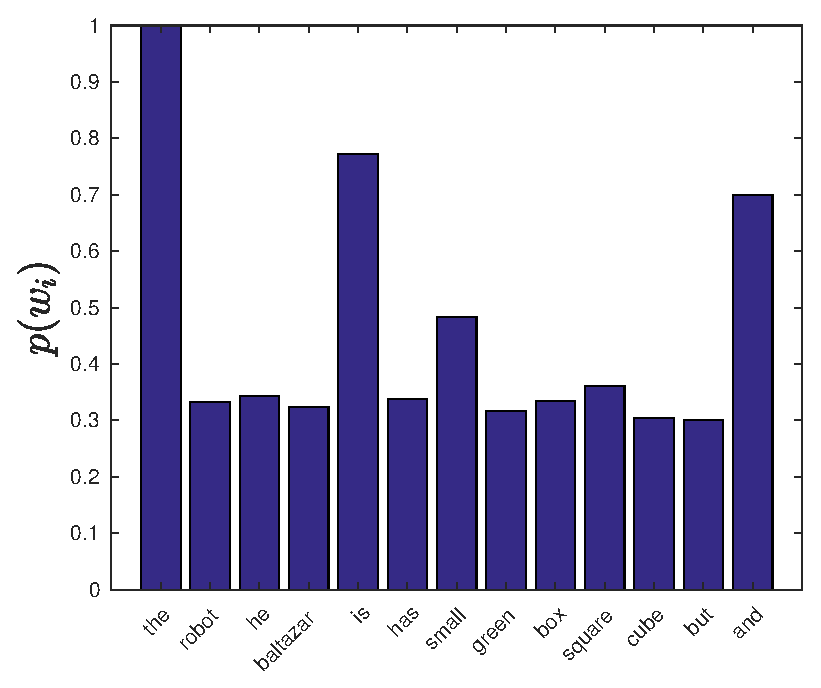
\includegraphics[width=0.9\columnwidth]{but_pw.eps}
% \caption{Word occurrence probabilities given the evidence \emph{\{\evidenceProducingBut\}}. The conjunctions ``and'' and ``but'' have comparable probabilities, with the former being slightly higher. See also Tab.~\ref{tab:conjunction:but}. We have omitted words for which no significant probability was observed.}
% \label{fig:conjunction_but:pw}
% \end{figure}

%generated sentences in Fig.~\ref{tab:conjunction:but}

% A clarification is due: even though the conjunction ``and'' is still the most likely, the conjunction ``but'' has a comparable probability, given the observed evidence~(see Fig.~\ref{fig:conjunction_but:pw}).
% Even so, ``but'' was chosen in the highest-ranked sentence and in two more of the top-ten sentences~(see Tab.~\ref{tab:conjunction:but}).
% This result can be loosely interpreted as TODO

\begin{figure}
\centering
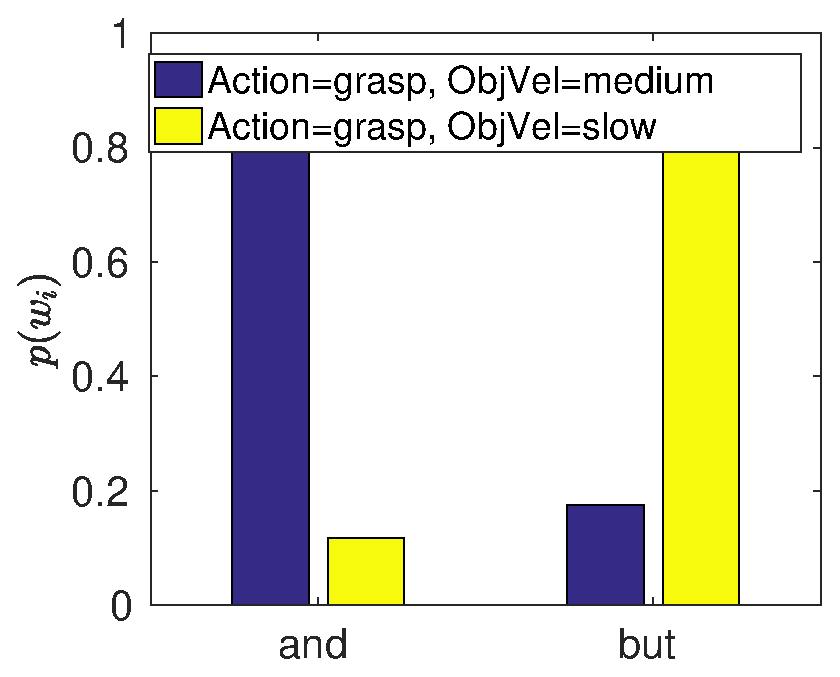
\includegraphics[width=0.9\columnwidth]{p_conjunctions.eps}
\caption{Word occurrence probabilities of the conjunctions ``and'' and ``but'' obtained when entering a consistent \actioneffect{} evidence vs when entering an inconsistent \actioneffect{} evidence. See Fig.~\ref{tab:conjunction} for details.}
\label{fig:p_conjunctions}
\end{figure}

\subsection{Solving Ambiguities with the Combined Model}

MOVE THIS RESULT EARLIER? (requires explanation of word probabilities, if we decide to include Fig.~\ref{fig:after_softevidence:pw})


Fig.~\ref{fig:update_from_softevidence} shows the result of predictions over nodes given some initial evidence, before and after incorporating further soft evidence

\begin{figure*}
    \centering
    \subfloat[][Prediction of the model given the initial (hard) evidence. The prediction is ambiguous.]
    { 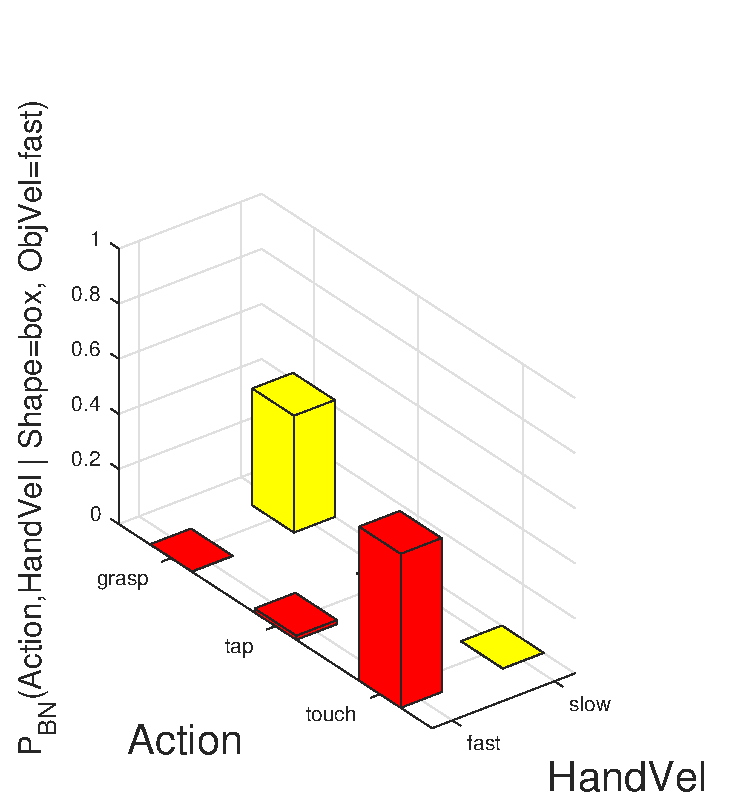
\includegraphics[width=0.45\linewidth]{before_softevidence_prediction.eps} \label{fig:before_softevidence:pred} } \quad
    %
    \subfloat[][Updated prediction of the model after having incorporated the Action soft evidence (grasp tap touch)=(0.8 0.1 0.1) TODO IMPROVE NOTATION. The prediction is now unambiguous.]
    { 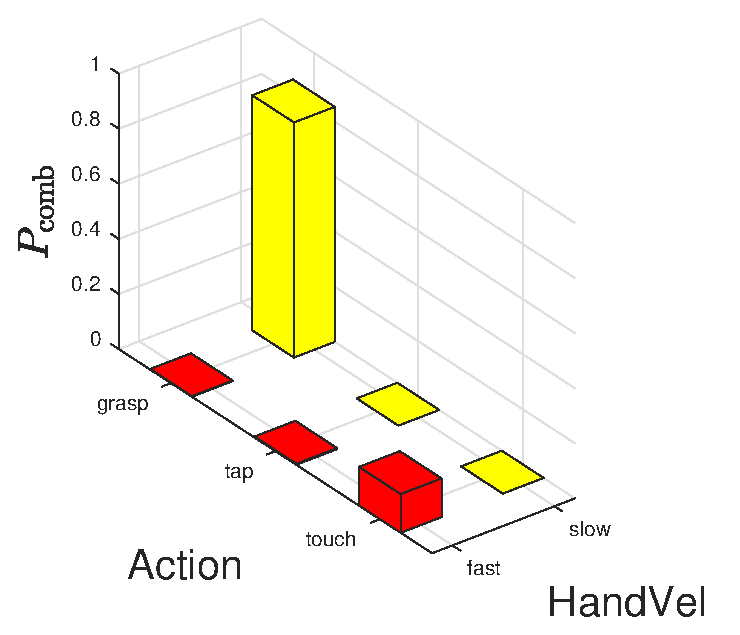
\includegraphics[width=0.45\linewidth]{after_softevidence_prediction.eps} \label{fig:after_softevidence:pred} }
    \caption{Predictions about the action and hand velocity on a box object, before and after incorporating Action soft evidence from Gesture \acp{HMM}.}
    \label{fig:update_from_softevidence}
\end{figure*}

word probabilities: Fig.~\ref{fig:after_softevidence:pw} (in this case they are identical before and after incorporating the soft evidence) REMOVE THIS?

\begin{figure}
\centering
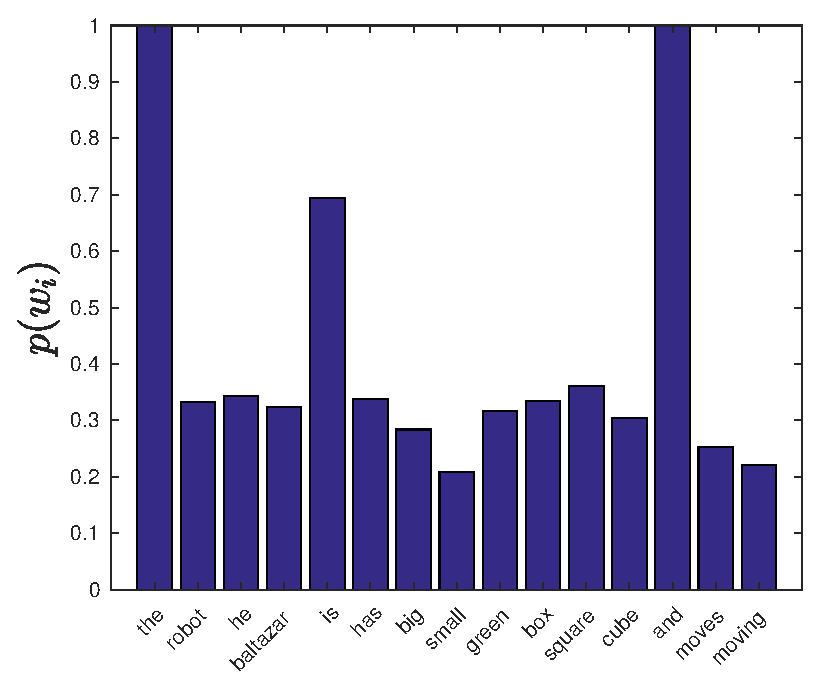
\includegraphics[width=0.9\columnwidth]{after_softevidence_pw.eps}
\caption{Word occurrence probabilities given the evidence \{Shape=box, ObjVel=fast\}. We have omitted words for which no significant probability was observed.}
\label{fig:after_softevidence:pw}
\end{figure}
